\chapter{Introduction} % Main chapter title
\label{chp:introduction} 

\todo{numbers!}
I should through some number about could-computing, DRM, and IoT widespread. 
(intuitively) What problems they have and whyin which scenario they are used 
and \emph{why}, what problem do they resolve?

\todo{Definition of TEE and usage. Properties, memory isolation, and remote 
attestation.}

\todo{History of TEEs, first definition, standard used, etc. During the 
description, stay "high level" and recall properties and differences. This 
should give a context.} 

\todo{Focus on SGX, explain the reason (widespread adoption, becoming standard, 
solutions are very tailored to a technology).}

\todo{General architecture of SGX, explain how it works and what you can and 
cannot do Figure~\ref{fig:sgx-architecture}.}

\todo{Motivations from Figure~\ref{fig:mind-map}, carry my reasoning and, at 
each point state explicitly what's the problem.}
\todo{Define 4 areas: (1) Anti-tampering (find a better name), (2) New threats, 
(3) Runtime RA, (4) Memory forensic. These are taken from the mind-map. For 
each class, state the problem clearly and list the contribution. Do it in 
separate subsections.}

\todo{State the \emph{thesis} of the thesis, and the "test" to falsify the 
thesis.}
My thesis argues that Trusted Execution Environments (TEE), such as SGX, are 
powerful tools that isolate portion of code against strong adversaries (\ie the 
OS itself).
However, TEEs are not the silver-bullet of cyber security and they suffer of 
limitations in terms of scalability and security.

I argue that we can further extend the TEE properties by carefully choosing 
smarter software design without the need of changing the TEE modules (and thus 
changing the hardware).
Throughout the dissertation, I first investigate the TEE limitations, 
then, I will propose relative solutions.
\todo{I have to discuss every point carefully, this is just a memory for me.}

\todo{Wrap up the limitations from the previous point, and describe the 
contribution of the thesis in Figure~\ref{fig:contribution}.}

%\todo{Introduction context of Trusted Execution Environments}
%Trusted Execution Environments (TEE) refers to set of technologies that 
%guarantee confidentiality and integrity of specific portion of code.
%\todo{Claim the properties they achieve}
%TEE are implemented at hardware level, such as at microcode for Intel 
%SGX~\todo{cite}, and allows one to define isolated portion of memory in which 
%executing critical piece of software and data, called \emph{enclaves}.
%The \emph{enclaves} are de-fact isolated sub-systems that work parallely with, 
%and isolated from, the other system components.
%Historically, Open Mobile Terminal Platform (OMTP) defined the TEE security 
%guarantees in \todo{cite}, and they define two level of security from attacker 
%\emph{software} and \emph{hardware}.
%For what concerns \emph{software} attacks, a TEE guarantees that other 
%software 
%component cannot directly read or write the \emph{enclave} memory space;
%while the \emph{hardware} defense extends this protection also against 
%manually 
%tampering with the hardware itself.
%Besides local protection, TEE implements Remote Attestation (RA) schemes
%that allow a remote entity, called \emph{Verifier}, to verify the identify and 
%integrity of a so-called \emph{Prover} (which is called \emph{enclave} in TEE 
%terminology).
%\todo{Few examples of applications}
%Such technology have been well adopted in many scenarios that vary from Web 
%applications to Digital Rights Managements (DRM) but also in embedding systems 
%or crypto currencies.
%\todo{Focus on a technology? Dunno...}
%Moreover, the commercial competition of TEE vendors (\eg Intel or AMD) 
%improved 
%the sophistication of \emph{enclaves} and smoothed the learning curve.
%As a result, nowadays it is easier to adopt TEE technologies in commercial 
%products.
%
%\todo{Focus on some of the new challenges}
%The new protections introduced by TEE rose the bar for attackers, that now 
%have 
%to face new challenges.
%Nonetheless, TEE technologies still suffer of many limitations in terms of 
%security and scalability.
%In this thesis, I will first describe modern TEE technolgies and the 
%challenges 
%that are not yet addressed (Chapter~\ref{chp:background}).
%From this step, I will study the limitations of current TEE works under 
%different point of view and propose mitigation to strengthen the 
%\emph{enclave} security properties.
%\todo{List the stuff I am going to touch}

\begin{figure}[t]
	\centering
	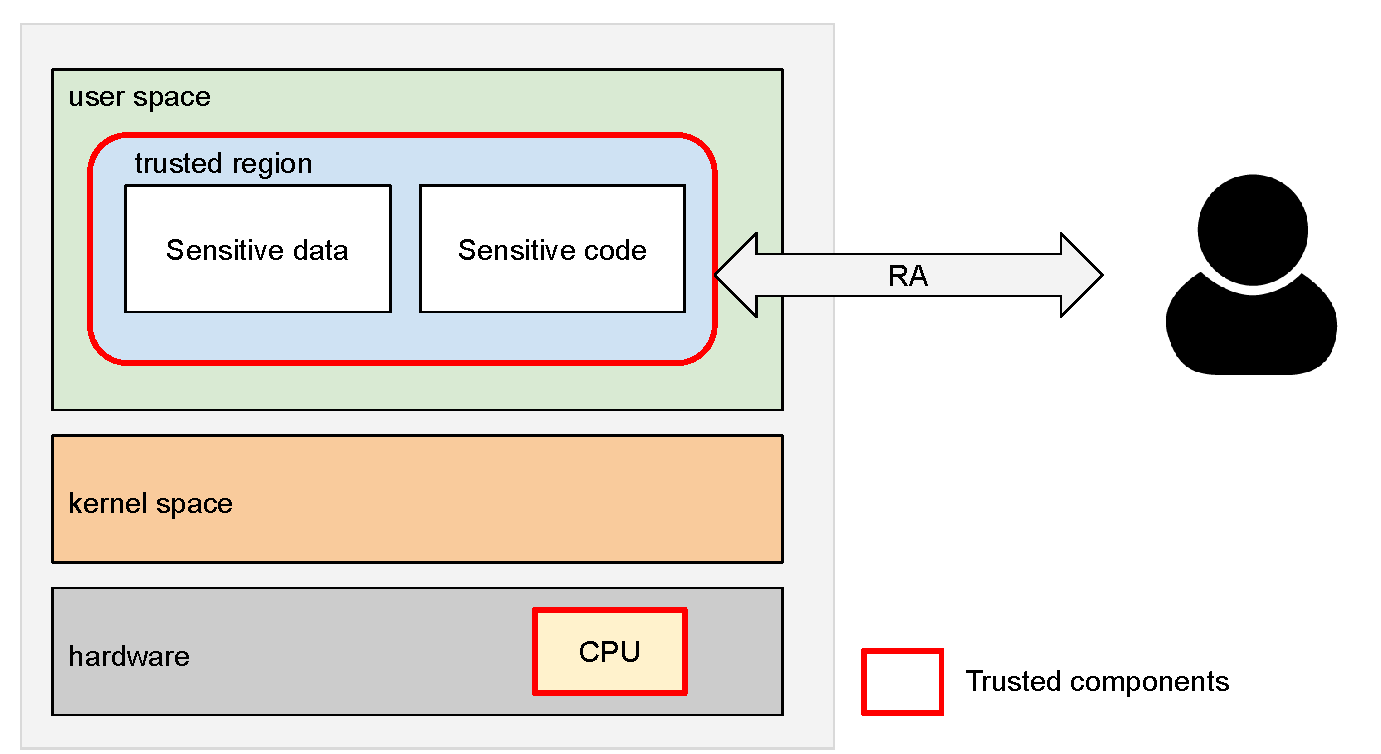
\includegraphics[width=0.5\textwidth]{fig_c1/sgx-architecture.pdf}
	\caption[SGX architecture.]{Simplified SGX architecture.}
	\label{fig:sgx-architecture}
\end{figure}

\begin{figure}[t]
	\centering
	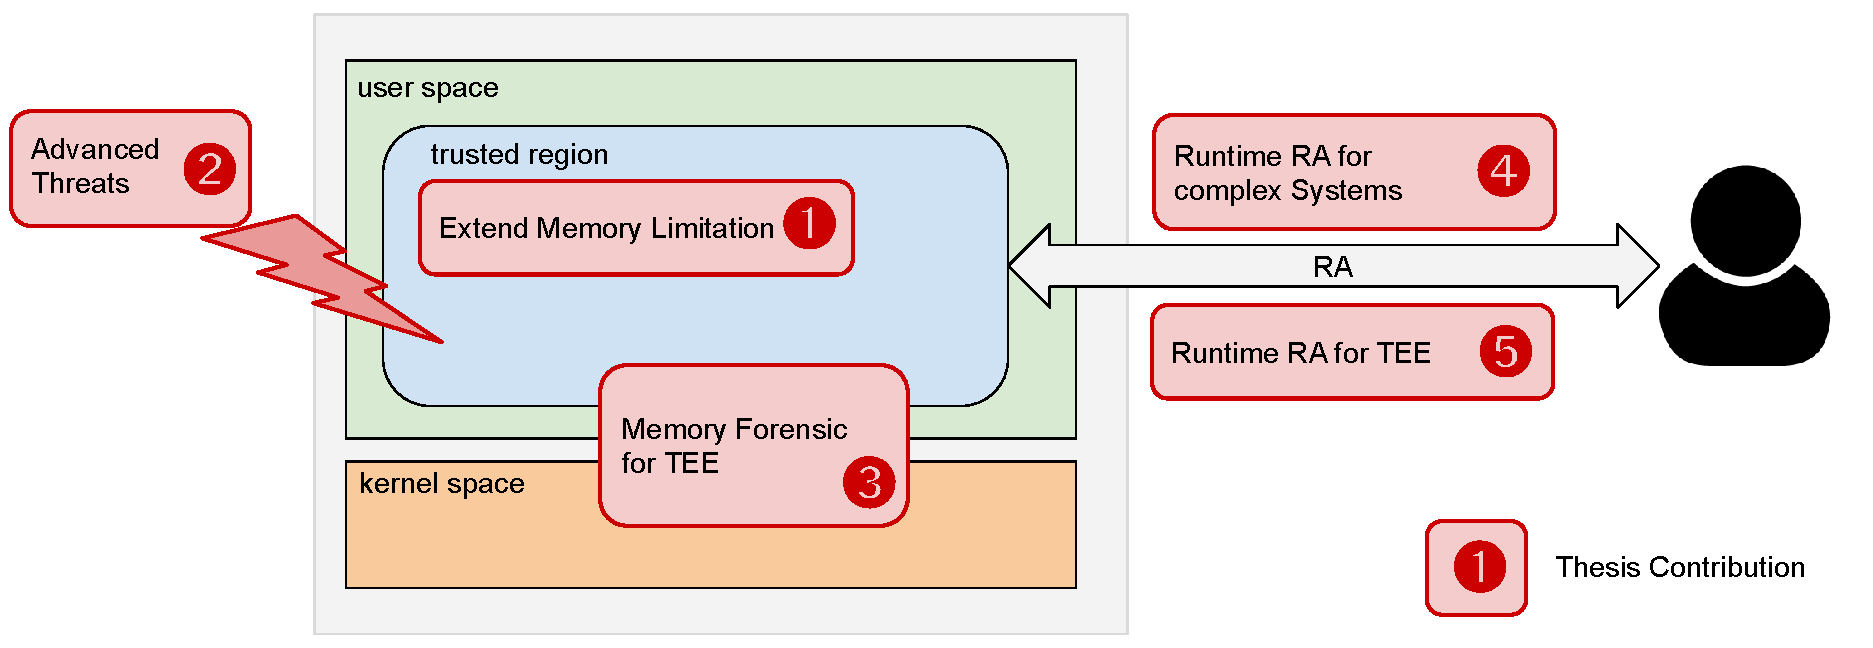
\includegraphics[width=0.7\textwidth]{fig_c1/contribution.pdf}
	\caption[Thesis contribution.]{Thesis contribution.}
	\label{fig:contribution}
\end{figure}

\begin{figure}[t]
	\centering
	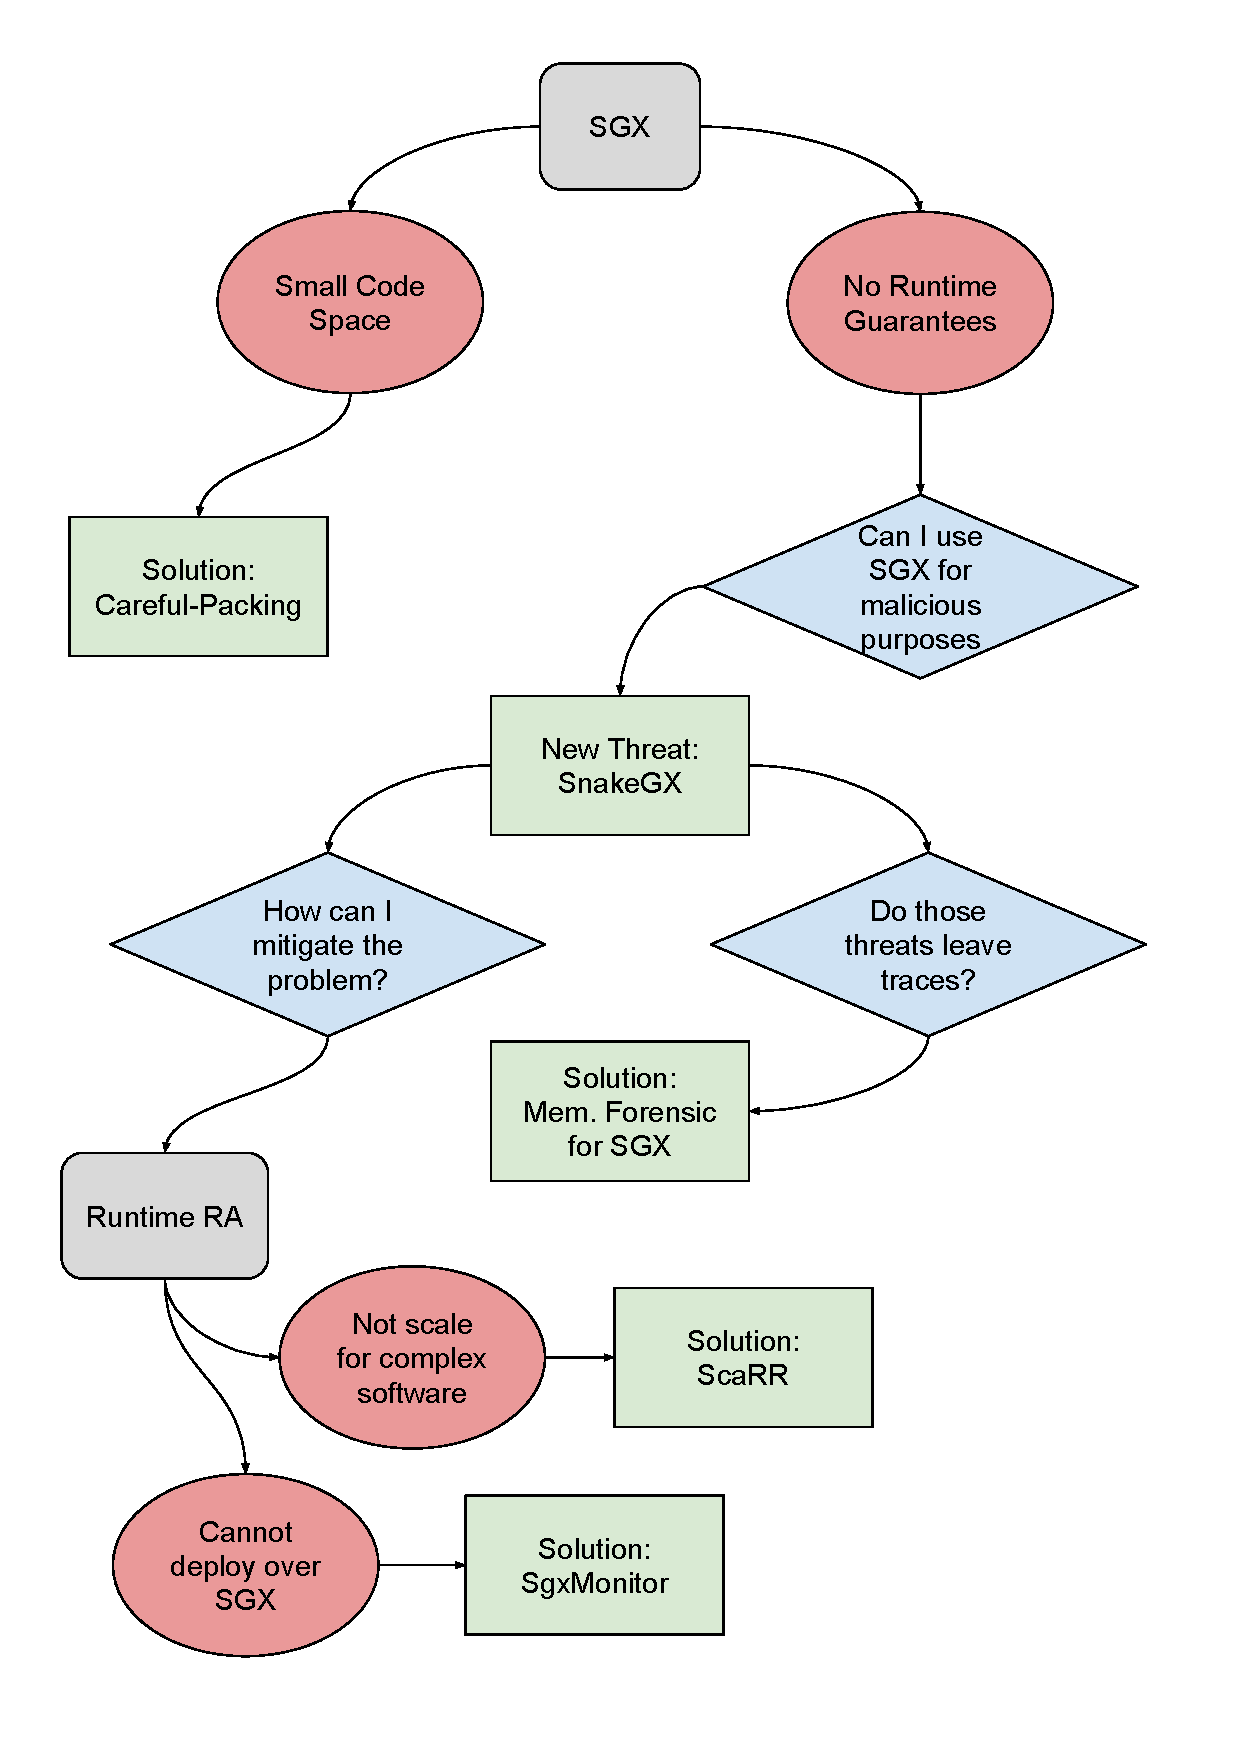
\includegraphics[width=\textwidth]{fig_c1/mind-map.pdf}
	\caption[Mind-map.]{Mind-map (TO REMOVE LATER).}
	\label{fig:mind-map}
\end{figure}


Overall, my study covers five TEE aspect:
\begin{itemize}
	\item \todo{Scalability untrusted code protection} First, I will face a 
	scalability issues that affect many modern	TEE technologies 
	(Chapter~\ref{chp:static-protection}).
	
	\item \todo{New threats} At this point, I covered static and runtime 
	protection for the untrusted code, now I will investigate new type of 
	threats for the \emph{enclaves} themselves 	
	(Chapter~\ref{chp:advanced-threats}).
	
	\item \todo{New defenses for the untrusted code} Then. I will use TEE to 
	implement runtime protection for untrusted memory 
	(Chapter~\ref{chp:runtime-protection-untrusted}).
	
	\item \todo{New defenses for the trusted code} From this point, I will 
	design new defenses for TEE \emph{encalves} 	
	(Chapter~\ref{chp:runtime-protection-trusted})
	
	\item \todo{Forensic analysis} Finally, I will investigate the new 
	challenges introduced by TEE technologies in terms of memory-forensic 
	analysis (Chapter~\ref{chp:forensic}).
\end{itemize}

